\chapter{Web Workers APIa}\index{Web Workers API}
Orain arte, JavaScript erabiliz hari bakarreko programak sortu ditugu. Web Worker APIak JavaScript scriptak aldi berean exekutatzeko ahalmena ematen digu. Hau oso interesgarria da konputazio handiko prozesuak lantzeko. Web Worker-ak existituko ez balira, arazo bat izango genuke, konputazio astun horiek egitean nabigatzailearen interfaze grafikoa blokeatu egingo litzatekeelako: hari bakar batek kalkuluak egin beharko lituzke eta aldi berean ezingo lituzke erabiltzailearen sarrerak kudeatu —saguarekin egindako mugimenduak, botoi-sakatzeak, etab.—.

Kasurik okerrenean nabigatzaileak errore-mezu bat pantailaratuko luke, skript batek kontrola hartu duela eta gainontzeko eragiketa guztiak blokeatu egin direla esateko, skripta amaitzeko aukera emanez (ikus \ref{fig:webworker1}. irudia).

\begin{figure}[ht]
	\centering
\begin{tikzpicture}
\node[anchor=south west,inner sep=0] (image) at (0,0)
   {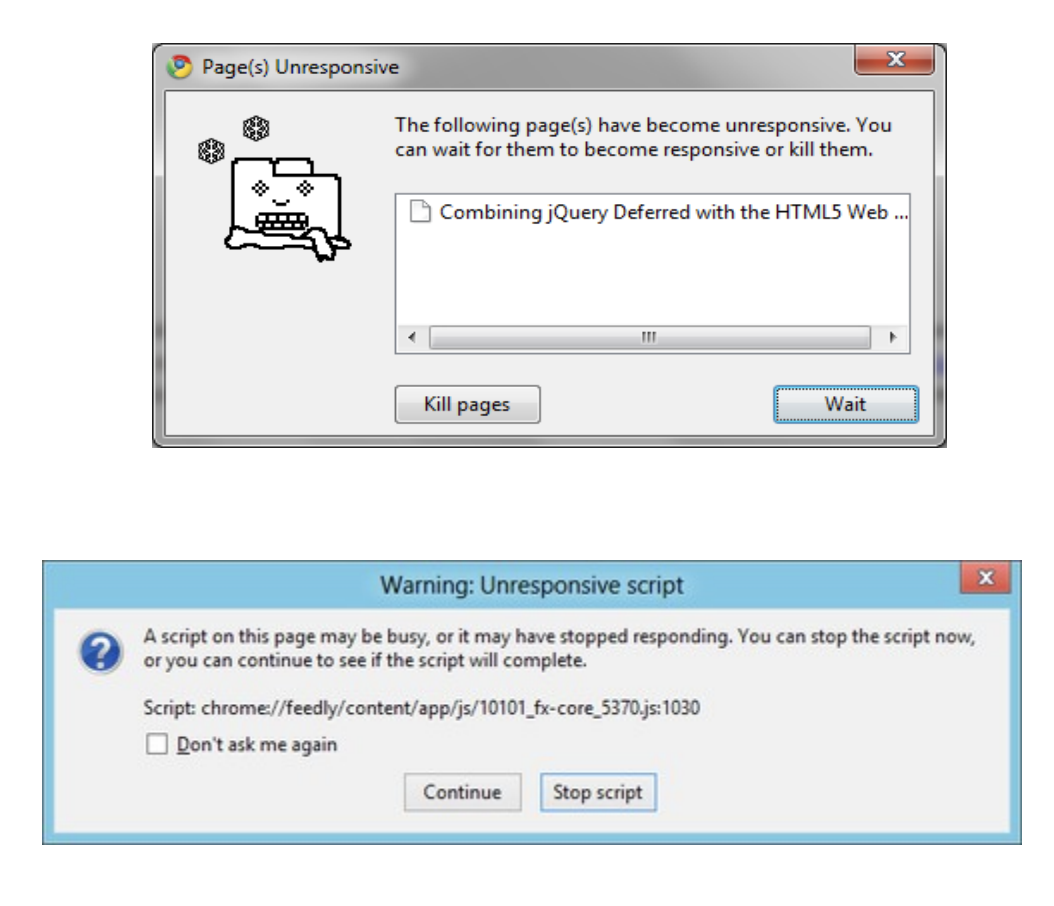
\includegraphics[trim=0cm 0cm 0cm 0cm, clip=true,
   width=0.5\textwidth]{img/page_unresponsive.png}};
\end{tikzpicture}
\caption{Nabigatzaileak exekuzio-denbora luzea behar duen skripta aurkitzen duenean, skript hori amaitu edo itxaroten jarraitu nahi dugun galdetuko digu. Web Worker APIak horrelako errore-mezuak ekiditen lagunduko digu.}
\label{fig:webworker1}
\end{figure}

Web Workers APIa bereziki garrantzitsua da RIA (\textit{Rich Internet Application}) aplikazioetan, aldi berean exekutatzen diren eragiketak egin nahi ditugulako, eta ziur asko horietako batzuk (edo asko) paraleloki egikaritu daitezkeelako, interfaze grafikoaren blokeoa saihestuz. API hau, web aplikazioen elkarreragin arina lortzeko, ezinbestekoa bilaka daiteke gure web aplikazioetan konputazio handiko eragiketak egin behar direnean.

Gai honetan ikusiko dugun Web Workers APIa erabiliz egindako adibideaz gain, John Resig \footnote{John Resig jQuery liburutegiaren sortzailea da. } programatzaileak bere blogean proposatzen dituenak ere aztertzea komeni da.\footnote{\href{http://ejohn.org/blog/web-workers/}{http://ejohn.org/blog/web-workers/}}

\section{Zer da Web Worker bat?}

Laburbilduz, Web Worker bat bigarren planoan exekutatzen den JavaScript programa bat da.

Erabiltzailearen interfaze grafikoa kudeatzen duen JavaScript haria blokeatu gabe, kalkulu-ahalmen handiko atazak exekutatzeko oso egokiak dira.

\section{Zer egin dezakegu Web Workers APIarekin?}

Web Worker-ak honako atazak sortzen dituzten kalkuluak egiteko aukera ezin hobeak dira, adibidez kasu hauetan: 
\begin{itemize}
    \item Jokoak, grafikoak, kriptografia...
    \item Sarrera/Irteera: URL bati \textit{polling} egiteko atzeko planoan.
    \item Web editoreetan erabiltzen den sintaxiaren koloreztatzea lortzeko.
    \item Bigarren planoan exekutatzen diren zuzentzaile ortografikoak.
    \item Online kalkulu-orriak  programatzeko.
    % \item      https://testdrive-archive.azurewebsites.net/Graphics/WorkerFountains/Default.html
    % \item https://msdn.microsoft.com/library/jj635756.aspx (Mandelbrot Fraktalak)
    % \item http://ejohn.org/blog/web-workers
\end{itemize}


\section{Nola erabili Web Worker APIa}

Web Worker berri bat sortzeko \textit{Worker}\index{Worker} klasea instantziatuko dugu:

\begin{lstlisting}[numbers=none]
let worker = new Worker("worker_script.js");
\end{lstlisting}

Web Worker bati mezu bat bidaltzeko \textit{postMessage} metodoa erabiliko dugu \index{postMessage}:
\begin{lstlisting}[numbers=none]
worker.postMessage("Kaixo mundua!");
\end{lstlisting}

Web Worker batek bidaltzen dizkigun erantzunak kudeatu:


\begin{lstlisting}[numbers=none]
worker.onmessage = function(event) {
   console.log("Jasotako mezua: " + event.data);
   zerbaitEgin();
}
\end{lstlisting}


Web Worker bat amaitzeko, berriz, \textit{terminate}\index{terminate} metodoaz baliatuko gara:

\begin{lstlisting}[numbers=none]
worker.terminate();
\end{lstlisting}


\section{Oinarrizko adibidea}

Zenbaki lehenak kalkulatzen lagunduko digun Web Worker bat programatuko dugu adibide honetan.

Lehenengo, lehenaDa() funtzioa programatuko dugu, \hlc[lightgray]{worker.js} fitxategian\footnote{
Adibidearen kodea hemen aurkituko duzu: \href{https://ikasten.io/html5/webworkers/index.html}{https://ikasten.io/html5/webworkers/index.html}}.

\begin{lstlisting}[numbers=none,language=JavaScript]
// worker.js fitxategia
function lehenaDa(n) {
    if (n == 2) return true;
    for (var i = 2; i <= Math.sqrt(n); ++i) {
        if (n % i == 0) return false;
    }
    return true;
}

// amaigabeko begizta batean lehenaDa metodoari
// deitu, 1-etik aurrera dauden zenbaki lehenak
// kalkulatu eta programa nagusiari postMessage 
// erabiliz bidaliko dizkiona
for (var i = 1; ; i++)
    if (lehenaDa(i))
        postMessage(i)
\end{lstlisting}

Jarraian, \textit{worker}-a instantziatu eta \textit{onmessage} metodoaren bidez \textit{worker}-aren mezuak tratatuko ditugu:

\begin{lstlisting}[numbers=none,language=HTML]
<!doctype html>
<html>
<head>
 <title>Web Worker bakar batekin zenbaki lehenak kalkulatzeko adibidea</title>
</head>
<body>
 <p>Kalkulatutako zenbaki lehen handiena: <div id="result"></div></p>
 <script>
 let worker = new Worker('worker.js');
 
 worker.onmessage = function (event) {
       document.getElementById('result').innerHTML = event.data;
 };
 </script>
</body>
</html>
\end{lstlisting}

Aplikazioa martxan jarri eta zenbaki lehenak kalkulatzen dituen bitartean, saguarekin testuaren zati bat hauta dezakegu, nabigatzailearen fitxa itxi, edo nahi duguna egin (\ref{fig:webworker2}. irudia). Programa bera probatzen badugu\footnote{Programa bera, baina Web Worker-ak erabili gabe, hemen aurkituko duzu: \href{https://ikasten.io/html5/webworkers/index2.html}{https://ikasten.io/html5/webworkers/index2.html}. Adi, workerrak erabiltzen direnez, adibide honek nabigatzailea blokeatuko du!} baina Web Worker-ak erabili gabe, nabigatzailea nola blokeatzen den nabarituko dugu (eta kasurik okerrenean ez digu utziko ezta aplikazioaren emaitza ikusi ere  —\ref{fig:webworker3}. irudia—.

\begin{figure}[ht]
	\centering
\begin{tikzpicture}
\node[anchor=south west,inner sep=0] (image) at (0,0)
   {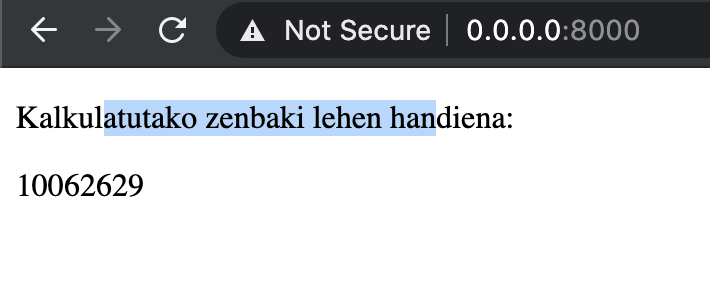
\includegraphics[trim=0cm 0cm 0cm 0cm, clip=true, width=0.5\textwidth]{img/webworkers/worker2.png}};
\end{tikzpicture}
\caption{Web Worker bat erabiliz posible da nabigatzailearekin lan egitea, kalkulu sakonak egiten diren bitartean.}
\label{fig:webworker2}
\end{figure}

\begin{figure}[ht]
	\centering
\begin{tikzpicture}
\node[anchor=south west,inner sep=0] (image) at (0,0)
   {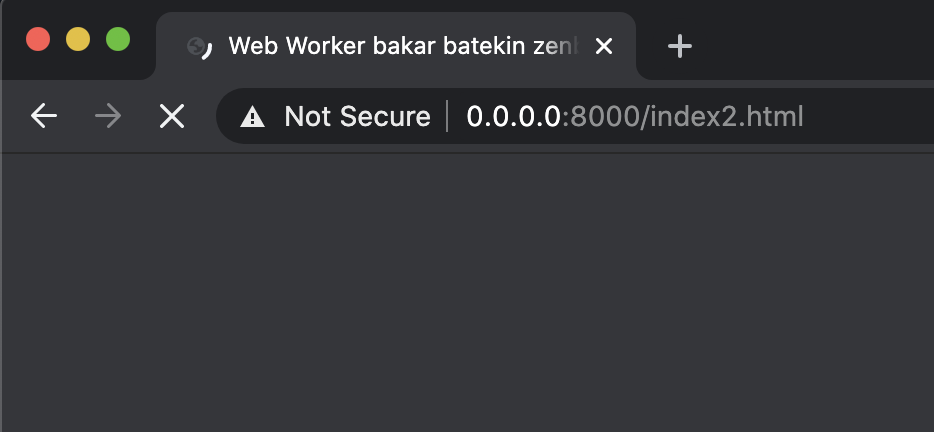
\includegraphics[trim=0cm 0cm 0cm 0cm, clip=true, width=0.5\textwidth]{img/webworkers/webworker3.png}};
\end{tikzpicture}
\caption{Web Worker APIa erabili gabe, orri nagusiak ez du kargatu ere egiten.}
\label{fig:webworker3}
\end{figure}

\section{Ariketak}
Ariketa bakar bat oraingo honetan. Web Worker APIa erabiltzeko \textit{script} baten berridazketa egitea eskatuko zaizu.  \href{https://ikasten.io/html5/webworkers/ww.html}{https://ikasten.io/html5/webworkers/ww.html} orrian dugun skriptak zenbaki lehenak kalkulatzen dituen bitartean \# karakterea inprimatzen du pantailan, behin eta berriro. Web Worker-ik erabiltzen ez duenez, kalkuluak egiten dituen bitartean nabigatzailea erdi blokeatuta geratzen da. Ariketa honen
eginbeharra kodea Web Worker APIa erabiltzeko moldatzea da.

%\href{https://flaviocopes.com/web-workers/}{Web Workers}

%\href{https://medium.freecodecamp.org/how-web-workers-can-help-with-consistent-asynchronous-tasks-in-javascript-cd6d728fa4ee}{How to use Web Workers to schedule consistent asynchronous tasks in JavaScript}

% \href{https://www.youtube.com/watch?v=X57mh8tKkgE}{WebWorkers: Code Session - Supercharged
%}